% !Mode:: "Tex:UTF-8"
\documentclass{xcumcmart}
\usepackage{setspace}
\usepackage{enumerate}
\usepackage{graphics}
\usepackage{tabu}

% \title{text}这里是显示在第三页的文章标题
\title{数据挖掘引论实验}
\author{何长鸿 2016141482154}

\linespread{1.2} %行距
% \setlength{\parskip}{1.2em} %1.4倍段落距离

\begin{document}
\renewcommand\arraystretch{2}
\maketitle
\section{数据准备}
\par 从http://archive.ics.uci.edu/ml/datasets/Wine下载数据集Wine,分别有wine.data和wine.names两个文件。根据arff格式语法,编辑整合得到wine.arff文件,部分内容如图\ref{fig:fg1}

\begin{figure}[htbp]
	\centering
	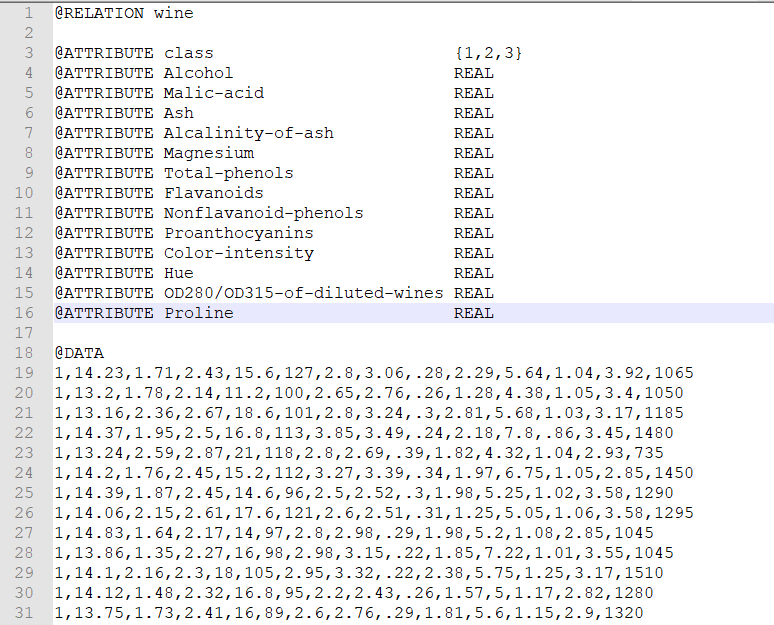
\includegraphics[width=0.8\textwidth]{fig/data.png}
    \caption{wine.arff数据内容\label{fig:fg1}}
\end{figure}

\section{预处理}
通过weka预处理页面观察数据集特征,可以看到红酒三个分类的数目分别为59,71,48。再观察变量与分类的相关可视化,如图\ref{fig:fg2},可以看到flavanoids、Hue等多个变量大小与红酒类别有明显的分层关系。
\begin{figure}[htbp]
	\centering
	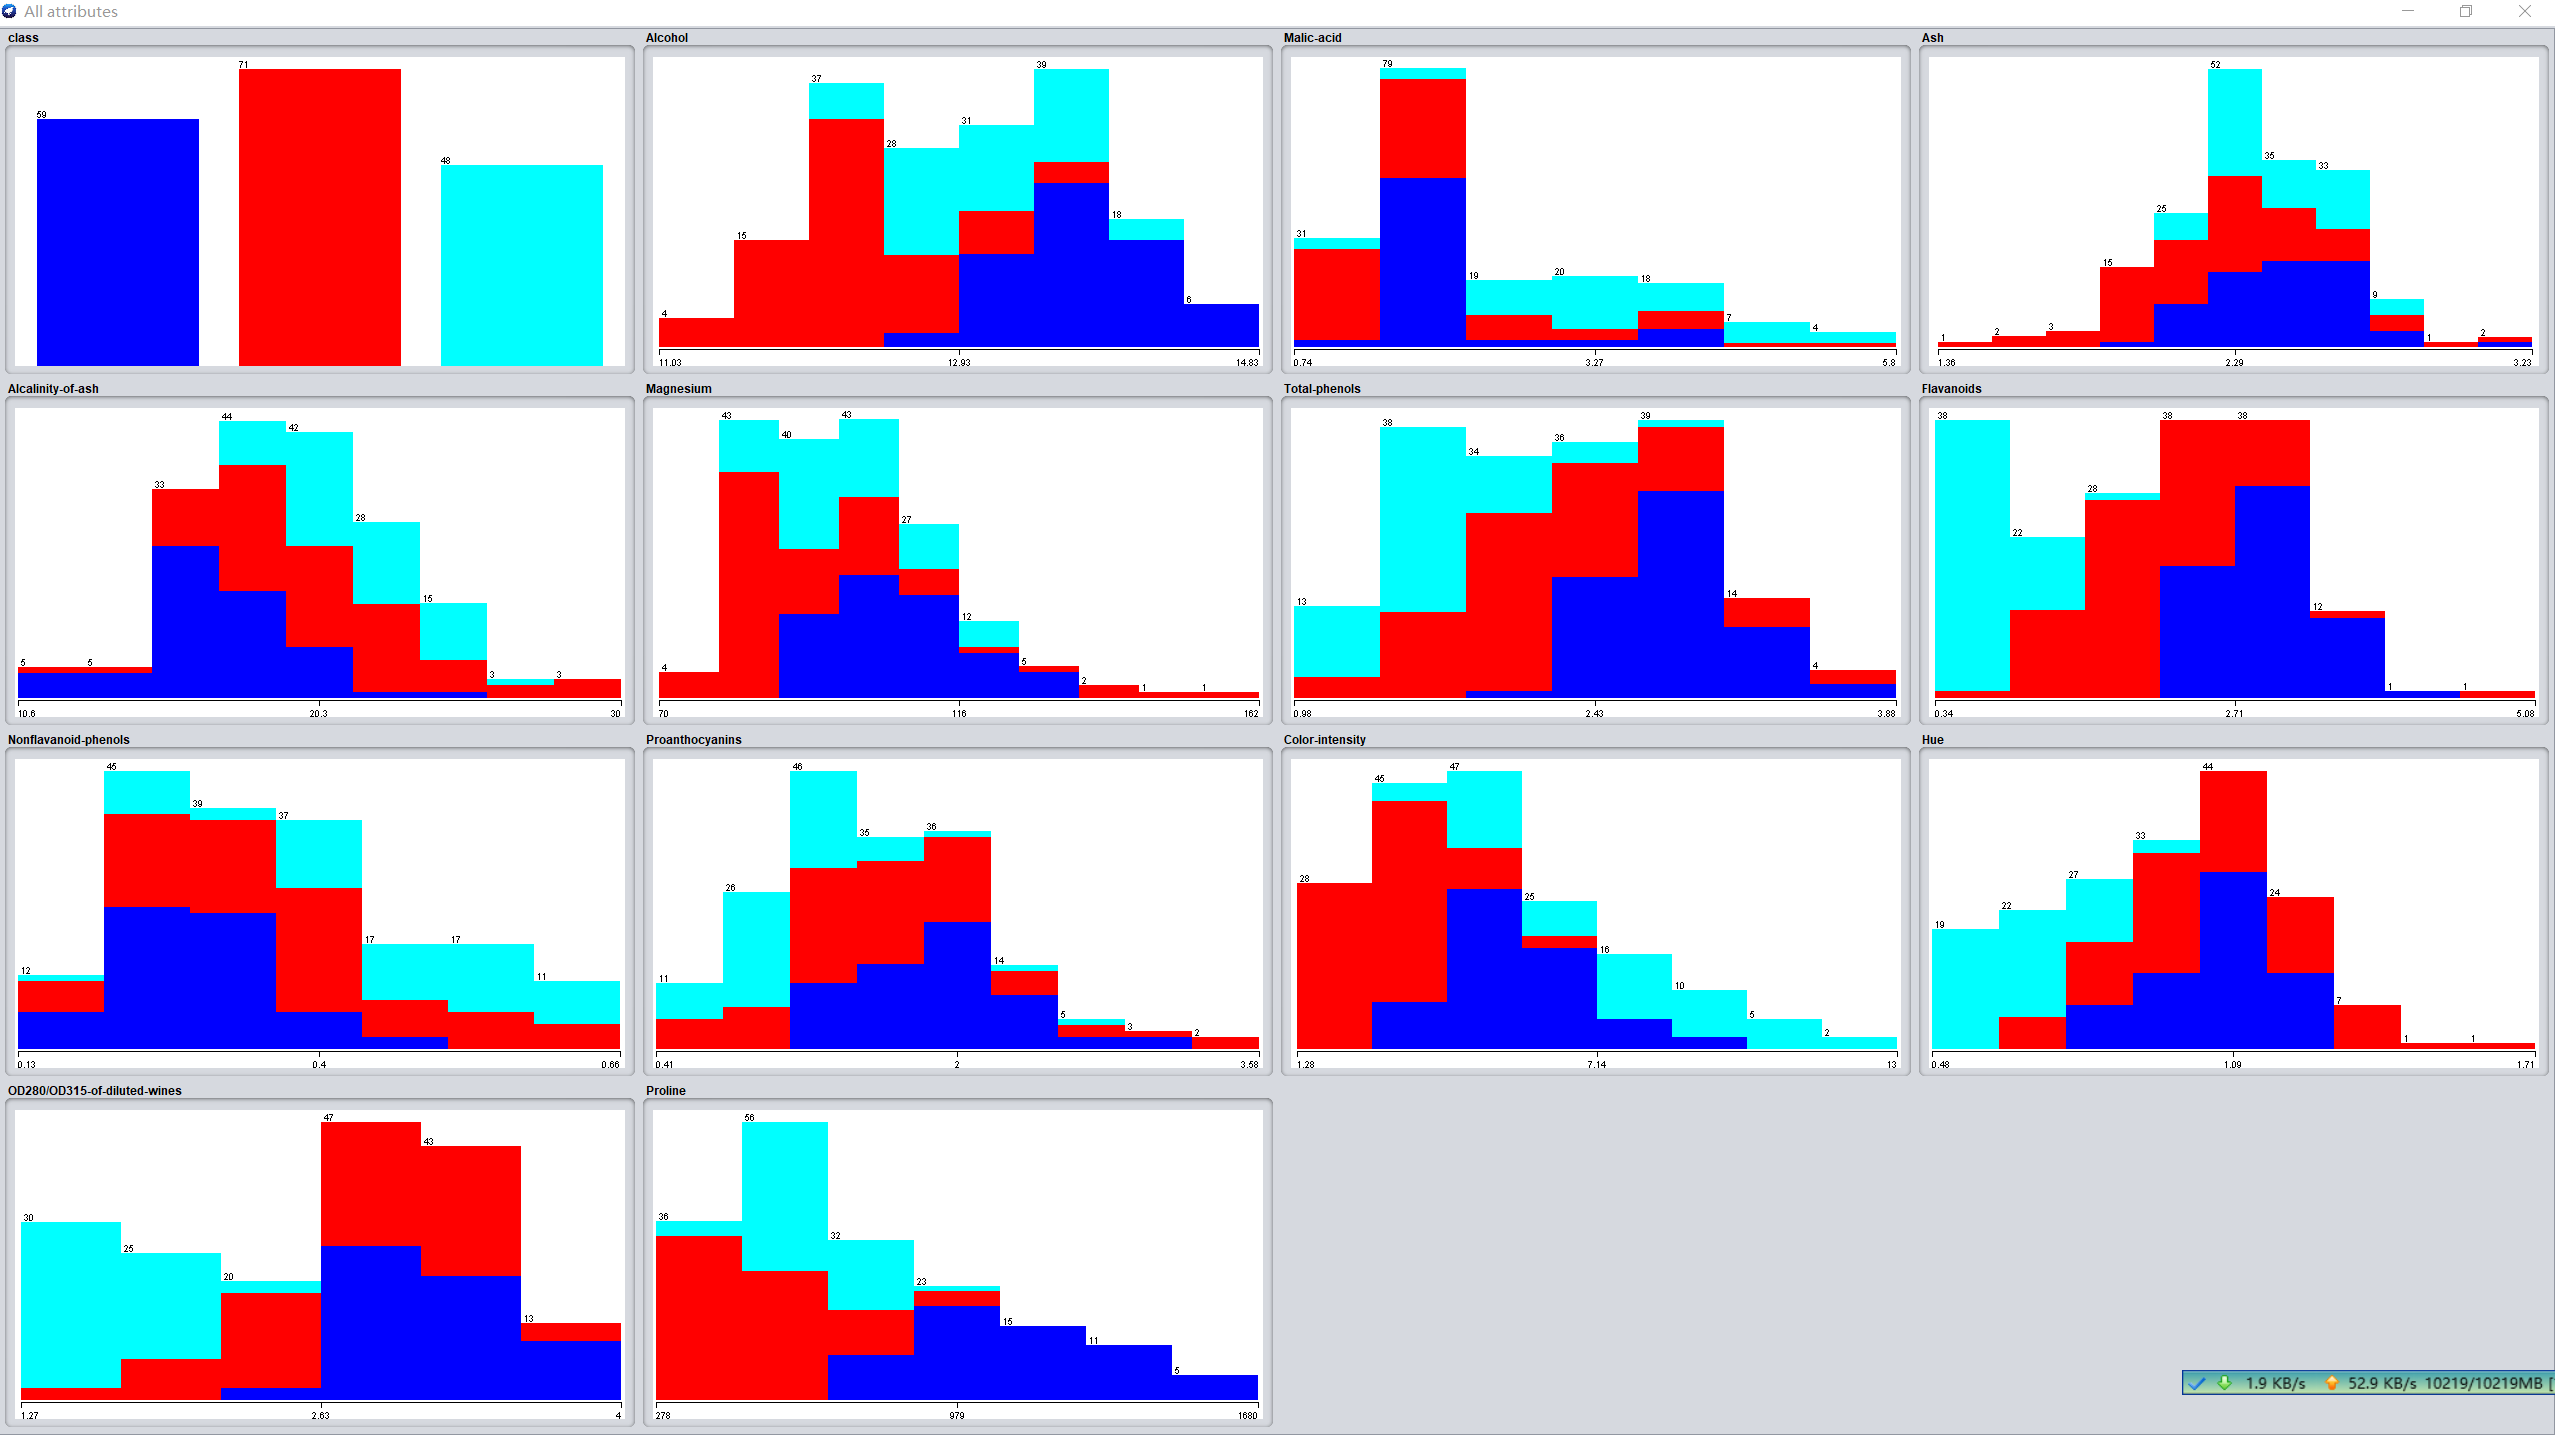
\includegraphics[width=0.8\textwidth]{fig/vis_data.png}
    \caption{数据分布\label{fig:fg2}}
\end{figure}
此外,各组变量均没有缺失值。
\section{分类}
先使用10-folds交叉验证测试模型,以及多种分类模型进行试验,得到多个预测结果,如图\ref{fig:fg3}、\ref{fig:fg4}分别为贝叶斯网和J48两种算法的运行结果,从混淆矩阵和各种分类评价指标来看,贝叶斯网取得了最好的分类结果。
\begin{figure}[htbp]
	\centering
	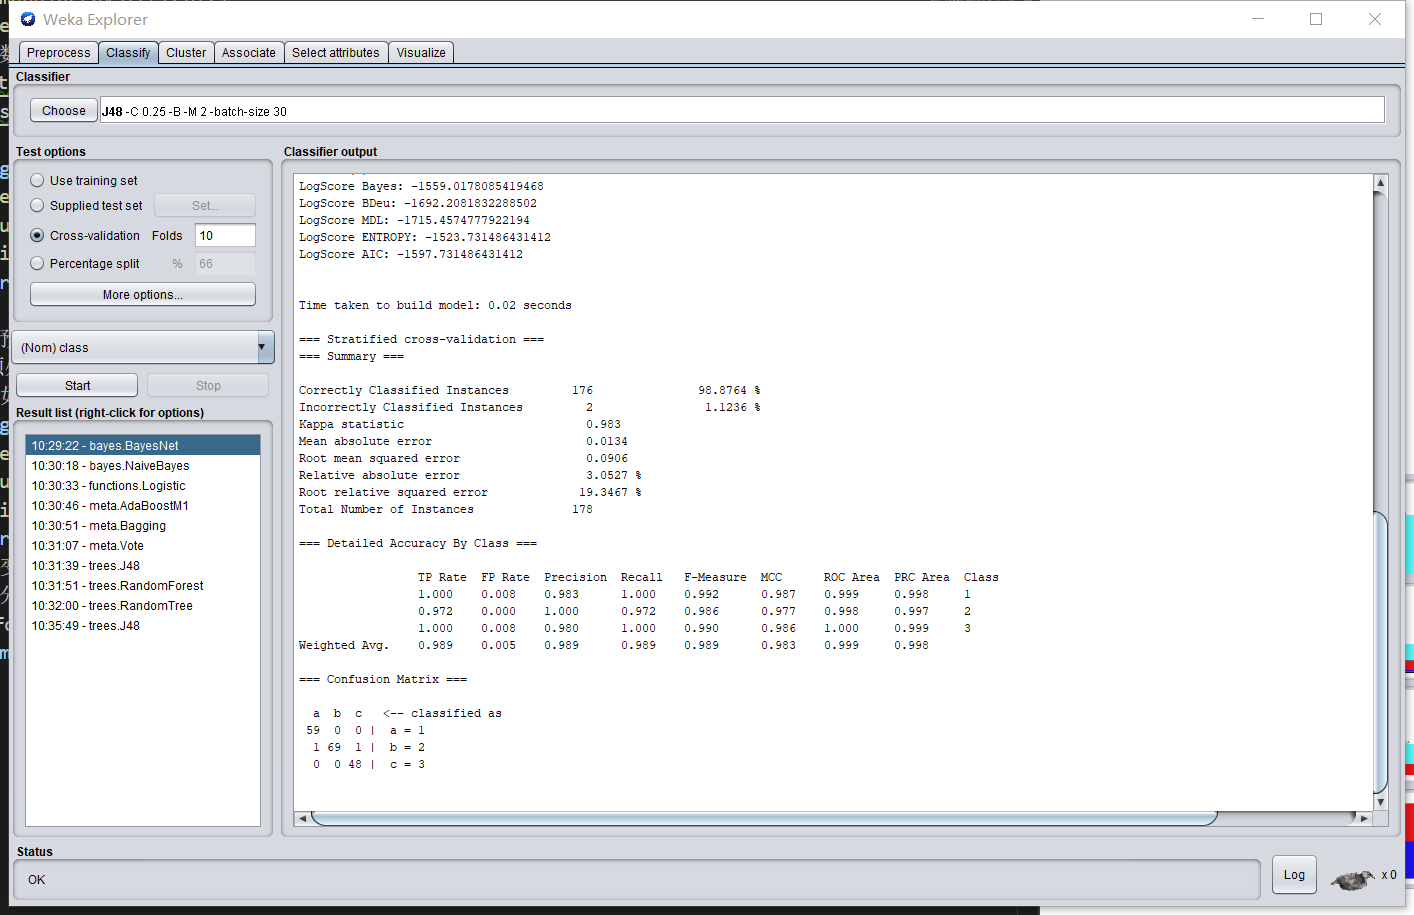
\includegraphics[width=0.8\textwidth]{fig/bayesnet.png}
    \caption{贝叶斯网\label{fig:fg3}}
\end{figure}
\begin{figure}[htbp]
	\centering
	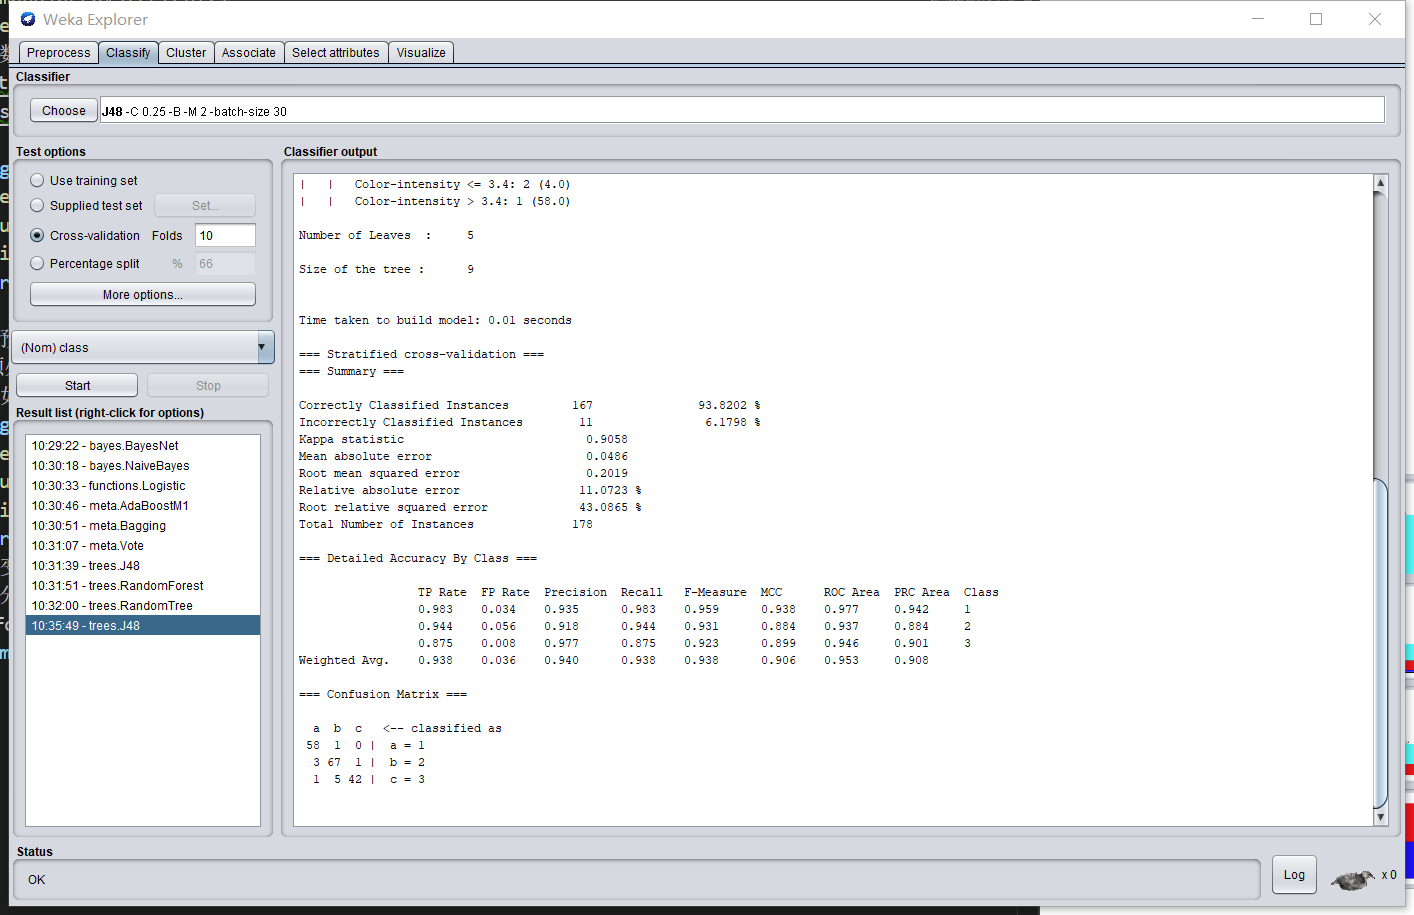
\includegraphics[width=0.8\textwidth]{fig/j48.png}
    \caption{J48\label{fig:fg4}}
\end{figure}
对以上两种模型结构进行可视化,得到如下图\ref{fig:fg5}、\ref{fig:fg6}
\begin{figure}[htbp]
	\centering
	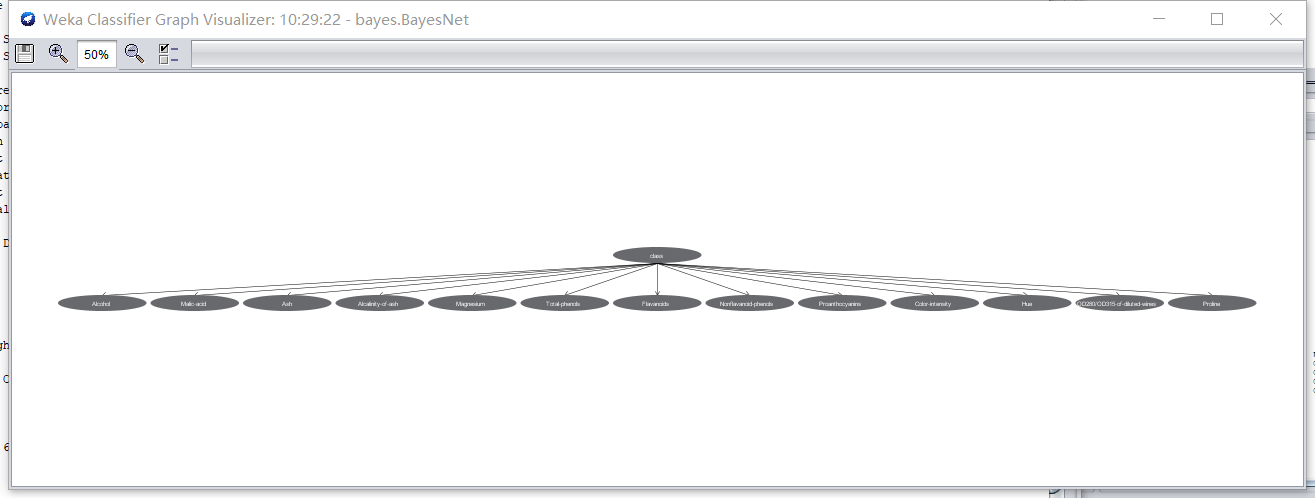
\includegraphics[width=0.8\textwidth]{fig/modelbayes.png}
    \caption{贝叶斯网模型结构\label{fig:fg5}}
\end{figure}
\begin{figure}[htbp]
	\centering
	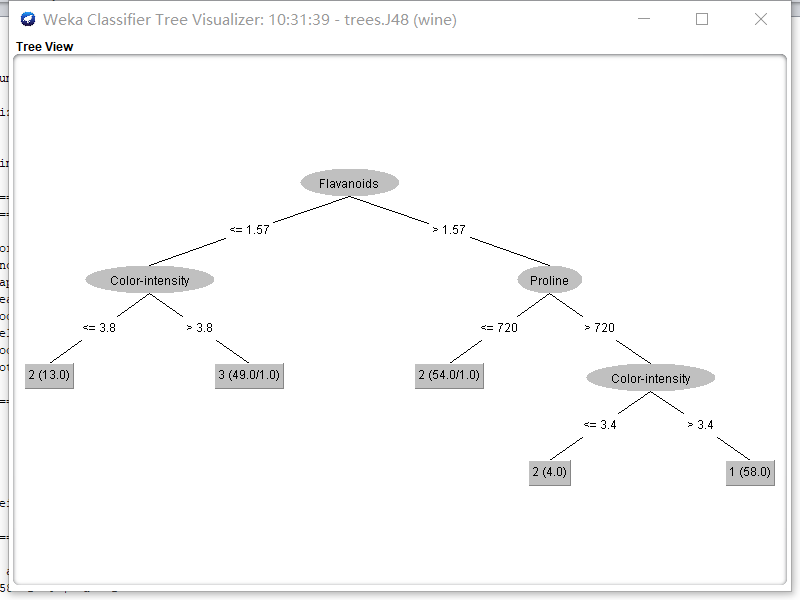
\includegraphics[width=0.8\textwidth]{fig/model_j48.png}
    \caption{J48树结构\label{fig:fg6}}
\end{figure}
\section{数据可视化}
通过wekaVisualize标签页面观察数据变量之间的相关关系,这里只选取了包括class在内的五个变量进行观察,如图\ref{fig:fg7}
\begin{figure}[htbp]
	\centering
	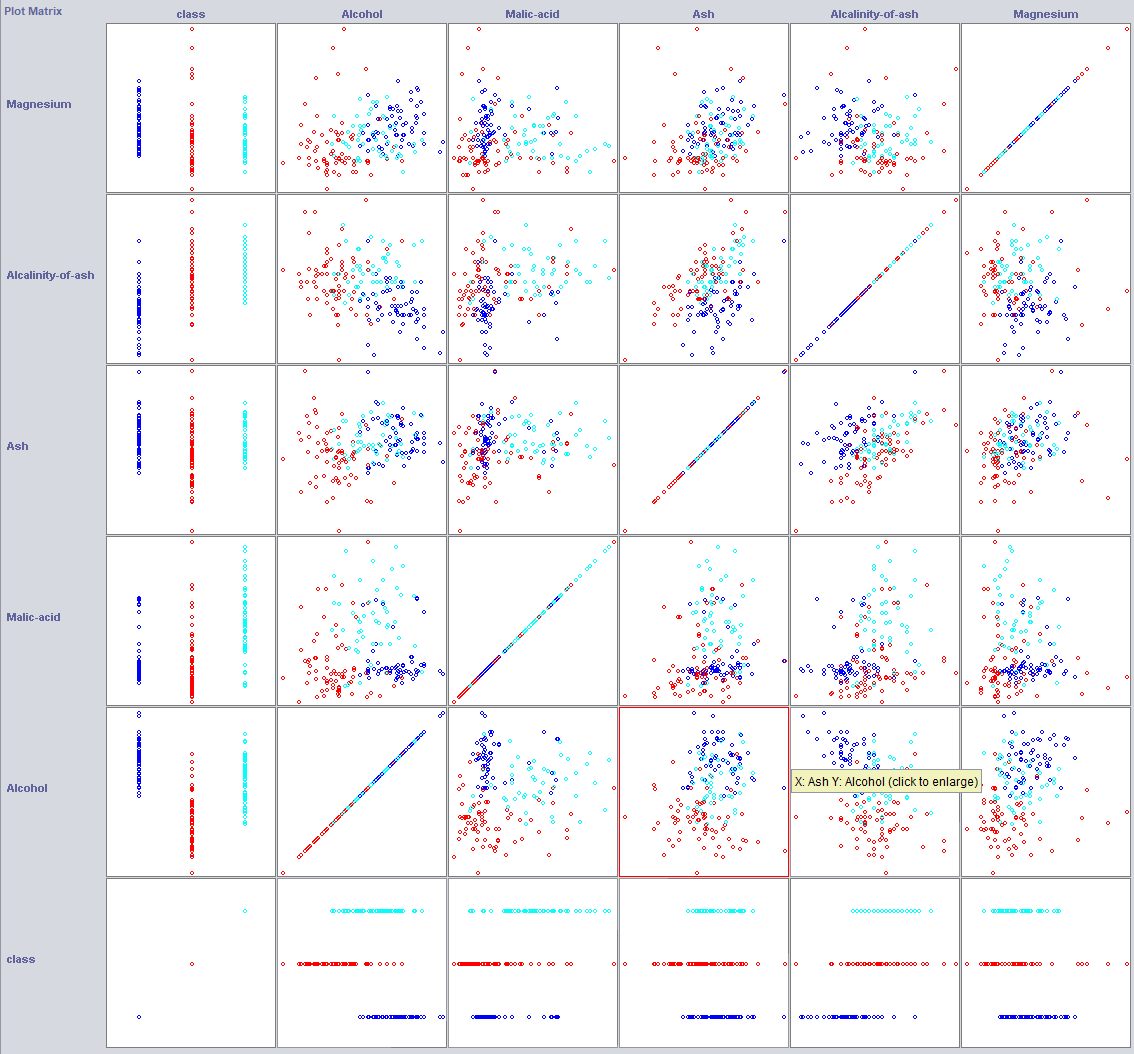
\includegraphics[width=0.8\textwidth]{fig/vis_all.png}
    \caption{变量关系\label{fig:fg7}}
\end{figure}
\end{document}